\documentclass[aspectratio=169,10pt]{beamer}

\usetheme{Madrid}
\usecolortheme{whale}
\setbeamertemplate{navigation symbols}{}
\setbeamertemplate{footline}[frame number]

\usepackage[T1]{fontenc}
\usepackage{lmodern}
\usepackage{booktabs}
\usepackage{tikz}
\usetikzlibrary{arrows.meta, positioning, shapes.geometric}

\definecolor{vgaccent}{RGB}{0,212,255}
\definecolor{vgdark}{RGB}{8,12,22}
\definecolor{vgpanel}{RGB}{14,20,36}

\setbeamercolor{structure}{fg=vgaccent}
\setbeamercolor{title}{fg=white,bg=vgdark}
\setbeamercolor{frametitle}{fg=white,bg=vgpanel}
\setbeamercolor{block title}{fg=white,bg=vgpanel}
\setbeamercolor{block body}{fg=black,bg=gray!8}

\title{Vector Vanguard}
\subtitle{Arcade Survival Shooter in C + SDL2}
\author{Pankaj}
\institute{Software Engineering Demo}
\date{\today}

\begin{document}

% --- Slide 1: Title (~30s) ---
\begin{frame}
  \titlepage
  \vspace{-0.5cm}
  \begin{center}
    \small \texttt{github.com/Pankaj809/vector-vanguard}
  \end{center}
\end{frame}

% --- Slide 2: Elevator pitch (~30s) ---
\begin{frame}{What Is Vector Vanguard?}
  \begin{block}{In plain English}
    You pilot a ship in a grid arena. Red enemies chase you.
    Shoot them before they hit you. Survive and score points.
  \end{block}
  \vspace{0.4cm}
  \begin{columns}[T]
    \column{0.5\textwidth}
    \textbf{Genre}
    \begin{itemize}
      \item Single-player arcade shooter
      \item Top-down survival
      \item 3 difficulty levels
    \end{itemize}
    \column{0.5\textwidth}
    \textbf{Built with}
    \begin{itemize}
      \item C99 + SDL2
      \item 1024$\times$768 display
      \item Sound + music + HUD log
    \end{itemize}
  \end{columns}
\end{frame}

% --- Slide 3: How to play (~45s) ---
\begin{frame}{How to Play}
  \begin{table}
    \centering
    \begin{tabular}{@{}ll@{}}
      \toprule
      \textbf{Action} & \textbf{Keys} \\
      \midrule
      Move ship       & WASD or Arrow keys \\
      Fire laser      & Space or Left Ctrl \\
      Menu navigate   & Up / Down \\
      Confirm         & Enter \\
      Go back         & Esc \\
      \bottomrule
    \end{tabular}
  \end{table}
  \vspace{0.3cm}
  \begin{alertblock}{Goal}
    Destroy enemies (+10 points each). You have \textbf{3 lives}.
    Beat your \textbf{high score}. Don't let hostiles reach your ship.
  \end{alertblock}
\end{frame}

% --- Slide 4: Game screens (~30s) ---
\begin{frame}{Game Flow}
  \centering
  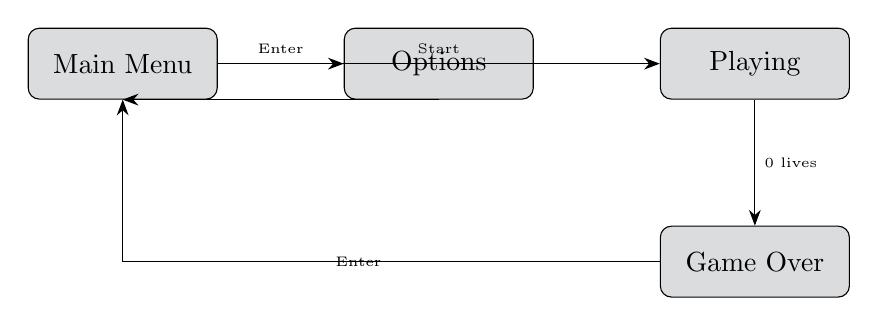
\begin{tikzpicture}[
    node distance=1.6cm,
    box/.style={draw, rounded corners, minimum width=2.4cm, minimum height=0.9cm, align=center, fill=vgpanel!15}
  ]
    \node[box] (menu) {Main Menu};
    \node[box, right=of menu] (opt) {Options};
    \node[box, right=of opt] (play) {Playing};
    \node[box, below=of play] (over) {Game Over};
    \draw[-{Stealth[length=2mm]}] (menu) -- node[above]{\tiny Enter} (opt);
    \draw[-{Stealth[length=2mm]}] (menu) -- node[above]{\tiny Start} (play);
    \draw[-{Stealth[length=2mm]}] (play) -- node[right]{\tiny 0 lives} (over);
    \draw[-{Stealth[length=2mm]}] (over.west) -| node[pos=0.25,left]{\tiny Enter} (menu.south);
    \draw[-{Stealth[length=2mm]}] (opt.south) |- (menu.south);
  \end{tikzpicture}

  \vspace{0.5cm}
  \small
  \textbf{Difficulty} (Options): Easy = slower enemies; Hard = faster spawns.
\end{frame}

% --- Slide 5: MVC overview (~45s) ---
\begin{frame}{Architecture: MVC Pattern}
  \begin{center}
  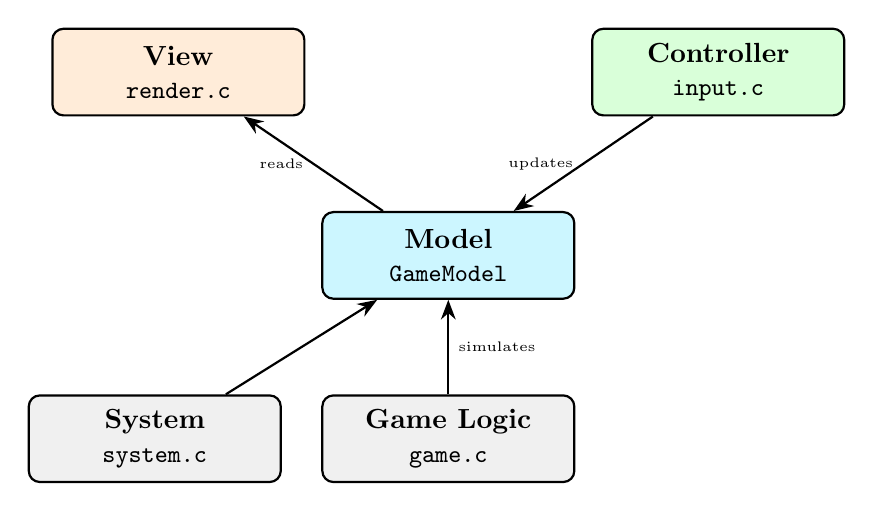
\begin{tikzpicture}[
    comp/.style={draw, thick, rounded corners, minimum width=3.2cm, minimum height=1.1cm, align=center},
    arr/.style={-{Stealth[length=2.5mm]}, thick}
  ]
    \node[comp, fill=vgaccent!20] (model) {\textbf{Model}\\\small\texttt{GameModel}};
    \node[comp, fill=orange!15, above left=1.2cm and 0.2cm of model] (view) {\textbf{View}\\\small\texttt{render.c}};
    \node[comp, fill=green!15, above right=1.2cm and 0.2cm of model] (ctrl) {\textbf{Controller}\\\small\texttt{input.c}};
    \node[comp, fill=gray!12, below=1.2cm of model] (logic) {\textbf{Game Logic}\\\small\texttt{game.c}};
    \node[comp, fill=gray!12, below left=1.2cm and 0.5cm of model] (sys) {\textbf{System}\\\small\texttt{system.c}};

    \draw[arr] (ctrl) -- node[left]{\tiny updates} (model);
    \draw[arr] (logic) -- node[right]{\tiny simulates} (model);
    \draw[arr] (model) -- node[left]{\tiny reads} (view);
    \draw[arr] (sys) -- (model);
  \end{tikzpicture}
  \end{center}

  \vspace{0.2cm}
  \small One struct (\texttt{GameModel}) holds \textbf{all game state}. Modules never own duplicate data.
\end{frame}

% --- Slide 6: Model (~30s) ---
\begin{frame}{The Model: \texttt{GameModel}}
  \begin{columns}[T]
    \column{0.55\textwidth}
    \textbf{Stores everything:}
    \begin{itemize}
      \item Screen state (menu, playing, game over)
      \item Score, lives, difficulty
      \item Player, enemies, bullets (entities)
      \item Particle effects
      \item Combat log messages
      \item Audio + font handles
    \end{itemize}
    \column{0.45\textwidth}
    \begin{block}{Why one model?}
      Easy to reason about.\\
      Easy to test.\\
      No hidden global variables.
    \end{block}
    \begin{exampleblock}{Memory pool}
      Up to 512 entities pre-allocated --- no malloc during gameplay.
    \end{exampleblock}
  \end{columns}
\end{frame}

% --- Slide 7: View \& Controller (~45s) ---
\begin{frame}{View vs Controller}
  \begin{columns}[T]
    \column{0.5\textwidth}
    \begin{block}{View --- \texttt{render.c}}
      \begin{itemize}
        \item Draws grid + HUD
        \item Renders ship, enemies, bullets
        \item Shows menus \& combat log
        \item \textbf{Never} changes game rules
      \end{itemize}
    \end{block}
    \column{0.5\textwidth}
    \begin{block}{Controller --- \texttt{input.c}}
      \begin{itemize}
        \item Reads keyboard
        \item Menu selection
        \item Moves player velocity
        \item Fires bullets
        \item \textbf{Never} draws pixels
      \end{itemize}
    \end{block}
  \end{columns}
  \vspace{0.3cm}
  \centering
  \small \texttt{main.c} runs the loop: \textbf{Input $\rightarrow$ Update $\rightarrow$ Render} at 60 FPS
\end{frame}

% --- Slide 8: Game logic layman (~45s) ---
\begin{frame}{Game Logic (Simple Terms)}
  \begin{enumerate}
    \item \textbf{Spawn} --- Every few seconds a new enemy appears at the top.
    \item \textbf{Chase} --- Each enemy moves toward your ship.
    \item \textbf{Shoot} --- Your bullets fly in the direction you last moved.
    \item \textbf{Hit test} --- Circles overlap? Enemy dies (+10) or you lose a life.
    \item \textbf{Respawn} --- Still have lives? Ship returns to center.
    \item \textbf{Game Over} --- No lives left; high score saved to disk.
  \end{enumerate}
  \vspace{0.2cm}
  \begin{block}{Fair physics}
    Game updates in fixed \textbf{1/60 second} steps so speed is identical on every computer.
  \end{block}
\end{frame}

% --- Slide 9: Engineering highlights (~30s) ---
\begin{frame}{Engineering Highlights}
  \begin{itemize}
    \item \textbf{Separation of concerns} --- MVC modules in separate \texttt{.c} files
    \item \textbf{Deterministic loop} --- Accumulator pattern in \texttt{main.c}
    \item \textbf{Asset pipeline} --- Fonts \& audio loaded via \texttt{system.c}
    \item \textbf{Portable build} --- CMake + \texttt{run.sh} for one-command start
    \item \textbf{Standalone deploy} --- \texttt{package.sh} bundles binary + assets
  \end{itemize}
\end{frame}

% --- Slide 10: Close (~15s) ---
\begin{frame}{Summary \& Demo}
  \begin{center}
    {\Large Vector Vanguard}\\[0.4cm]
    Arcade fun + clean C architecture\\[0.6cm]
    \textbf{Clone \& play:}\\
    \texttt{git clone https://github.com/Pankaj809/vector-vanguard.git}\\
    \texttt{./run.sh}\\[0.6cm]
    \textbf{Questions?}
  \end{center}
\end{frame}

\end{document}
